
	\documentclass{article}
	\usepackage{amsmath,amssymb}
	\usepackage[inline]{enumitem}
	\usepackage{blindtext}
	\usepackage{booktabs}
	\usepackage{graphicx}
	\usepackage{xcolor}
	\usepackage[vmargin = 1.5in, top = 1in, bottom = 1.2in, letterpaper]{geometry}
	\usepackage{listings}
	\usepackage{courier}
	\usepackage{multicol}
	\usepackage{multirow}
	\usepackage{bm}
	\usepackage{subcaption}
	\usepackage{tabularx}
	\usepackage{fancyvrb}
	\lstset{
	basicstyle = \small\tt,
	keywordstyle = \tt\color{blue},
	commentstyle = \it\color[cmyk]{1,0,1,0},
	stringstyle = \tt\color[RGB]{128,0,0},
	%frame = single,
	backgroundcolor = \color[RGB]{245,245,244},
	breaklines,
	extendedchars = false,
	xleftmargin = 2em,
	xrightmargin = 2em,
	aboveskip = 1em,
	tabsize = 4,
	showspaces = false
	}
    \newenvironment{CVerbatim}{\center\BVerbatim}{\endBVerbatim\endcenter}
	\begin{document}
	
	% \newfontfamily\courier{Courier New}


	
	\title{STAT 557 Final Exam}
	\author{Yifan Zhu}
	\maketitle
	
	\section{Problem 1: Danish Alcohol Consumption Study}
	\subsection{Summary of findings}
	In this study, we find alcohol consumption is always associated with income, marriage and urbanization under any constraints. However, the association between alcohol consumption and urbanization does not depend on income and marriage status, and we find in higher urbanized area people tend to drink more. When conditioning on different marriage status, the association between alcohol consumption changes, but common points are people with income over 100,000 Dkr tend to drink more than people with lower income, and among high income people, people with income over 150,000 Dkr tend to drink less than people with income between 100,000 - 150,000 Dkr.

	\subsection{Description of methods used}
	First we fit a complete independent model by assuming 
	\[\log(m_{ijkl}) = \lambda_{i}^A + \lambda^C_j + \lambda_{k}^B + \lambda^D_l\]
	Then the goodness of fit test for this model is
		\begin{verbatim}
                Pearson test =  1733.46
          Degrees of freedom =  168
                     p-value =  0
               Deviance test =  1503.76
                          df =  168
                     p-value =  0 
		\end{verbatim}

    We can see the p-value is pretty small. So the complete independent model does not seem to be a good choice. Then we used \verb|step| function in R to find a model starting with the full model. Then the model it returns is
    \[\log(m_{ijkl}) = \lambda_{i}^A + \lambda_{j}^C + \lambda_{k}^B + \lambda_{l}^D + \lambda_{ij}^{AC} + \lambda_{ik}^{AB} + \lambda_{il}^{AD} + \lambda_{jk}^{CB} + \lambda_{jl}^{CD} + \lambda_{kl}^{BD} + \lambda_{ijk}^{ACB}\]
    The AIC is 1042.248 and the result of goodness of fit test is
    \begin{verbatim}
                Pearson test =  155.3
          Degrees of freedom =  112
                     p-value =  0.00427
               Deviance test =  160.8
                          df =  112
                     p-value =  0.00173 
    \end{verbatim}

    The fit is not good from the result, so we look at the model only without the 4-way interaction and see its goodness of fit. The AIC is 1072.108, and the results of goodness of fit test is
    \begin{verbatim}
                Pearson test =  55.33
          Degrees of freedom =  48
                     p-value =  0.21746
               Deviance test =  62.66
                          df =  48
                     p-value =  0.07593 
    \end{verbatim}

    It is better in fitting the data, but the model is a lot more complex than the stepwise selected one. And the ANOVA of this model is
             \begin{verbatim}
               Df Deviance Resid. Df Resid. Dev  Pr(>Chi)    
         NULL                    179     8268.4              
         A      2  1014.22       177     7254.2 < 2.2e-16 ***
         C      3  1289.60       174     5964.6 < 2.2e-16 ***
         B      2  3061.08       172     2903.5 < 2.2e-16 ***
         D      4  1399.79       168     1503.8 < 2.2e-16 ***
         A:C    6   224.42       162     1279.3 < 2.2e-16 ***
         A:B    4    86.40       158     1192.9 < 2.2e-16 ***
         A:D    8   198.53       150      994.4 < 2.2e-16 ***
         C:B    6   570.86       144      423.5 < 2.2e-16 ***
         C:D   12   100.43       132      323.1 4.591e-16 ***
         B:D    8   133.26       124      189.9 < 2.2e-16 ***
         A:C:B 12    29.05       112      160.8 0.0038681 ** 
         A:C:D 24    22.73        88      138.1 0.5358200    
         A:B:D 16    39.80        72       98.3 0.0008336 ***
         C:B:D 24    35.61        48       62.7 0.0598060 .  
         ---
         Signif. codes:  0 ‘***’ 0.001 ‘**’ 0.01 ‘*’ 0.05 ‘.’ 0.1 ‘ ’ 1
             \end{verbatim}
    From the table, it seems like we can try to drop the ACD interaction. So we drop the term and fit a model without 4-way interaction and ACD interaction. The ANOVA table is
    \begin{verbatim}
               Df Deviance Resid. Df Resid. Dev  Pr(>Chi)    
         NULL                    179     8268.4              
         A      2  1014.22       177     7254.2 < 2.2e-16 ***
         C      3  1289.60       174     5964.6 < 2.2e-16 ***
         B      2  3061.08       172     2903.5 < 2.2e-16 ***
         D      4  1399.79       168     1503.8 < 2.2e-16 ***
         A:C    6   224.42       162     1279.3 < 2.2e-16 ***
         A:B    4    86.40       158     1192.9 < 2.2e-16 ***
         A:D    8   198.53       150      994.4 < 2.2e-16 ***
         C:B    6   570.86       144      423.5 < 2.2e-16 ***
         C:D   12   100.43       132      323.1 4.591e-16 ***
         B:D    8   133.26       124      189.9 < 2.2e-16 ***
         A:C:B 12    29.05       112      160.8  0.003868 ** 
         A:B:D 16    30.54        96      130.3  0.015412 *  
         C:B:D 24    36.06        72       94.2  0.054150 .  
         ---
         Signif. codes:  0 ‘***’ 0.001 ‘**’ 0.01 ‘*’ 0.05 ‘.’ 0.1 ‘ ’ 1
    \end{verbatim}
    And the goodness of fit for this model is
    \begin{verbatim}
                     Pearson test =  87.08
               Degrees of freedom =  72
                          p-value =  0.10876
                    Deviance test =  94.2
                               df =  72
                          p-value =  0.04069 
    \end{verbatim}
    And the AIC is 1055.651. Although the p-value is larger than that of stepwise selected model, the p-value is still small. So the fit is not good and the AIC is larger than stepwise selected one. So we decide still use the stepwise selected model because it is simpler, which is
    \[\log(m_{ijkl}) = \lambda_{i}^A + \lambda_{j}^C + \lambda_{k}^B + \lambda_{l}^D + \lambda_{ij}^{AC} + \lambda_{ik}^{AB} + \lambda_{il}^{AD} + \lambda_{jk}^{CB} + \lambda_{jl}^{CD} + \lambda_{kl}^{BD} + \lambda_{ijk}^{ACB}\]
		\subsection{Final model and conclusions}

    The final model is
    \[\log(m_{ijkl}) = \lambda_{i}^A + \lambda_{j}^C + \lambda_{k}^B + \lambda_{l}^D + \lambda_{ij}^{AC} + \lambda_{ik}^{AB} + \lambda_{il}^{AD} + \lambda_{jk}^{CB} + \lambda_{jl}^{CD} + \lambda_{kl}^{BD} + \lambda_{ijk}^{ACB}\]

    The parameter estimates and standard errors are
    \begin{verbatim}
                     Estimate Std. Error z value Pr(>|z|)    
         (Intercept)  1.23856    0.27385   4.523 6.10e-06 ***
         A2          -0.53135    0.39677  -1.339 0.180511    
         A3          -0.79827    0.50903  -1.568 0.116830    
         C2           0.55744    0.31702   1.758 0.078678 .  
         C3          -0.35571    0.39064  -0.911 0.362511    
         C4           2.46630    0.27321   9.027  < 2e-16 ***
         B2           1.75450    0.25645   6.842 7.84e-12 ***
         B3          -0.25998    0.32678  -0.796 0.426277    
         D2          -1.17963    0.29018  -4.065 4.80e-05 ***
         D3          -0.43383    0.25417  -1.707 0.087844 .  
         D4           0.72703    0.20687   3.515 0.000441 ***
         D5           0.57192    0.21453   2.666 0.007676 ** 
         C2:B2        0.13288    0.28827   0.461 0.644814    
         C3:B2        0.23444    0.36787   0.637 0.523930    
         C4:B2       -1.93986    0.24513  -7.914 2.50e-15 ***
         C2:B3        0.52887    0.36694   1.441 0.149501    
         C3:B3        0.49383    0.46367   1.065 0.286846    
         C4:B3       -0.19848    0.31857  -0.623 0.533263    
         A2:C2       -0.09550    0.48665  -0.196 0.844417    
         A3:C2       -0.06551    0.62441  -0.105 0.916447    
         A2:C3        1.18191    0.52041   2.271 0.023140 *  
         A3:C3        0.27329    0.72688   0.376 0.706935    
         A2:C4        0.18737    0.40185   0.466 0.641025    
         A3:C4        0.05051    0.51992   0.097 0.922607    
         A2:D2        0.28111    0.13772   2.041 0.041227 *  
         A3:D2        0.13013    0.16287   0.799 0.424321    
         A2:D3        0.17596    0.13466   1.307 0.191319    
         A3:D3       -0.54237    0.17742  -3.057 0.002236 ** 
         A2:D4       -0.19090    0.11240  -1.698 0.089442 .  
         A3:D4       -0.78503    0.13917  -5.641 1.69e-08 ***
         A2:D5       -0.53180    0.11461  -4.640 3.49e-06 ***
         A3:D5       -1.17206    0.14652  -7.999 1.25e-15 ***
         B2:D2        0.65168    0.16866   3.864 0.000112 ***
         B3:D2       -0.25580    0.19498  -1.312 0.189542    
         B2:D3        1.07186    0.18920   5.665 1.47e-08 ***
         B3:D3        0.55791    0.20728   2.692 0.007112 ** 
         B2:D4        0.84456    0.14078   5.999 1.98e-09 ***
         B3:D4        0.19642    0.15542   1.264 0.206298    
         B2:D5        1.58544    0.15847  10.005  < 2e-16 ***
         B3:D5        0.84687    0.17331   4.887 1.03e-06 ***
         A2:B2       -0.33362    0.40315  -0.828 0.407934    
         A3:B2       -1.28462    0.55400  -2.319 0.020406 *  
         A2:B3        0.98359    0.47477   2.072 0.038291 *  
         A3:B3        0.65036    0.62665   1.038 0.299349    
         C2:D2        0.66128    0.27747   2.383 0.017160 *  
         C3:D2        1.03126    0.28453   3.624 0.000290 ***
         C4:D2        0.84301    0.26616   3.167 0.001539 ** 
         C2:D3       -0.15440    0.22181  -0.696 0.486375    
         C3:D3       -0.51081    0.24374  -2.096 0.036107 *  
         C4:D3       -0.31153    0.21224  -1.468 0.142146    
         C2:D4        0.16633    0.19487   0.854 0.393360    
         C3:D4        0.05405    0.20824   0.260 0.795213    
         C4:D4        0.07198    0.18525   0.389 0.697594    
         C2:D5       -0.24952    0.19083  -1.308 0.191026    
         C3:D5       -0.63161    0.20794  -3.037 0.002386 ** 
         C4:D5       -0.37131    0.18160  -2.045 0.040881 *  
         A2:C2:B2     0.88002    0.50232   1.752 0.079789 .  
         A3:C2:B2     1.19904    0.67413   1.779 0.075298 .  
         A2:C3:B2     0.25139    0.53810   0.467 0.640372    
         A3:C3:B2     1.72248    0.77171   2.232 0.025614 *  
         A2:C4:B2     0.91234    0.42097   2.167 0.030218 *  
         A3:C4:B2     1.68109    0.57678   2.915 0.003561 ** 
         A2:C2:B3    -0.14988    0.58382  -0.257 0.797389    
         A3:C2:B3     0.05846    0.76074   0.077 0.938748    
         A2:C3:B3    -0.52929    0.63916  -0.828 0.407616    
         A3:C3:B3     0.40422    0.87290   0.463 0.643312    
         A2:C4:B3    -0.21716    0.49501  -0.439 0.660878    
         A3:C4:B3     0.32171    0.65068   0.494 0.621004    
         ---
         Signif. codes:  0 ‘***’ 0.001 ‘**’ 0.01 ‘*’ 0.05 ‘.’ 0.1 ‘ ’ 1
    \end{verbatim}
    We can see any pair of daily alcohol consumption, income, marriage status and urbanization is associated from the model. Among income, marriage status and urbanization, as there is no three interaction term involving CD and BD, thus the association between income and urbanization and the association between marriage status and urbanization do not change with other variables changing. We collapse the contingency table of expected values and normalize to make the marriage status and income summing to 1, then we have
    \begin{center}
    	\begin{tabular}{lllllll}
    	\toprule
    	& \multicolumn{5}{c}{Unbanization}\\
Income &     1        &  2       &  3       &   4         &5\\
\midrule
1      & 0.08514493& 0.04071661 &0.1245791 &0.09348442 &0.1575046\\
2      & 0.23188406& 0.23127036 &0.3013468 &0.29405099 &0.3137739\\
3      & 0.16485507& 0.24592834 &0.1481481 &0.17450425 &0.1334157\\
4      & 0.51811594& 0.48208469 &0.4259259 &0.43796034 &0.3953057\\
    	\bottomrule
    	\end{tabular}
    \end{center}


        \begin{center}
    	\begin{tabular}{lllllll}
    	\toprule
    	& \multicolumn{5}{c}{Unbanization}\\
Marriage Status &     1        &  2       &  3       &   4         &5\\
\midrule
1 &0.2101449 &0.1482085 &0.09259259 &0.1212465 &0.06423718\\
2 &0.5217391 &0.7003257 &0.70538721 &0.7053824 &0.77269920\\
3 &0.2681159 &0.1514658 &0.20202020 &0.1733711 &0.16306362\\
    	\bottomrule
    	\end{tabular}
    \end{center}

    From the tables above, we find with higher level of urbanization, income level tends to be higher and marriage status tends to be less likely to be married, widow and unmarried probability go higher.

    In terms of the association between alcohol consumption and other 3 variables, we find there is no conditional independence for any pair of them, and the association between alcohol consumption and income would change when marriage status changes, and so does the association between alcohol consumption between marriage status when income changes. But the association would not change for different urbanization. Also, since there is no three way interaction term involving AD, the association between alcohol consumption and urbanization does not change with other variables changing.

    First, we examine the association between alcohol consumption and urbanization. By collapsing contingency table, we have
        \begin{center}
    	\begin{tabular}{lllllll}
    	\toprule
    	& \multicolumn{5}{c}{Unbanization}\\
Alcohol &     1        &  2       &  3       &   4         &5\\
\midrule
1& 0.3677536 &0.3078176 &0.3855219 &0.4600567 &0.55960469\\
2& 0.3985507 &0.4690554 &0.4848485 &0.4141643 &0.34342187\\
3& 0.2336957 &0.2231270 &0.1296296 &0.1257790 &0.09697344\\
    	\bottomrule
    	\end{tabular}
    \end{center}
    From the table we found with higher level of urbanization, alcohol consumption tends to be higher.

    Then we examine the association between alcohol consumption and income conditioning on different levels of marriage status.

    Condition on marriage status being widow:
        \begin{center}
    	\begin{tabular}{lllllll}
    	\toprule
    	& \multicolumn{4}{c}{Income}\\
Alcohol &     1        &  2       &  3       &   4     \\
\midrule
1& 0.5714286 &0.5806452 &0.3170732 &0.5180995\\
2& 0.2857143 &0.2741935 &0.5609756 &0.3303167\\
3& 0.1428571 &0.1451613 &0.1219512 &0.1515837\\
    	\bottomrule
    	\end{tabular}
    \end{center}

    We can see for widow, the income levels 0-50 and 50-100 do not have much difference in alcohol consumption, and for income level 100-150, people are more likely to take 1-2 units per day than other income levels. For income level 150 or above, people tend to drink more than first two income levels but not too much, and they are more likely to drink less than 1 unit per day than people in income level 100 - 150.

        Condition on marriage status being married:
        \begin{center}
    	\begin{tabular}{lllllll}
    	\toprule
    	& \multicolumn{4}{c}{Income}\\
Alcohol &     1        &  2       &  3       &   4     \\
\midrule
1& 0.72376874& 0.5164395 &0.3338008 &0.4170813\\
2& 0.23554604& 0.3857257 &0.5007013 &0.4336650\\
3& 0.04068522& 0.0978348 &0.1654979 &0.1492537\\
    	\bottomrule
    	\end{tabular}
    \end{center}

    For married people, we can see people tend to drink more with higher income level. But the people with income level being over 150 tend to drink less than people with income level being 100-150.   

            Condition on marriage status being unmarried:
        \begin{center}
    	\begin{tabular}{lllllll}
    	\toprule
    	& \multicolumn{4}{c}{Income}\\
Alcohol &     1        &  2       &  3       &   4     \\
\midrule
1& 0.37500 &0.4071856 &0.22 &0.3400000\\
2& 0.46875 &0.4131737 &0.57 &0.4333333\\
3& 0.15625 &0.1796407 &0.21 &0.2266667\\
    	\bottomrule
    	\end{tabular}
    \end{center}

        For unmarried people, we people with income level being 100-150 are more likely to drink 1-2 units per day than other levels. The probability of drinking more than 2 units per day for income level 100-150 and over 150 do not seem to have much difference, but the probability of drinking less than 1 unit for income level over 150 is higher than that of income level 100-150. So people in income level over 150 tend to drink less than people in income level 100 -150. 

	\subsection{Logistic regression model}
	When we subtract $\log(m_{1jkl})$ with $\log(m_{3jkl})$, all terms that do not involve A are canceled out. Then we have
	\begin{align*}
	\log\left(\frac{m_{1jkl}}{m_{3jkl}}\right) &= (\lambda_{1}^A - \lambda_{3}^A) + (\lambda_{1j}^{AC} - \lambda_{3j}^{AC}) + (\lambda_{1k}^{AB} - \lambda_{3k}^{AB}) + (\lambda_{1l}^{AD} - \lambda_{3l}^{AD}) + (\lambda_{1jk}^{ACB} - \lambda_{3jk}^{ACB})\\
		& = \mu_1 + \alpha_{j1} + \beta_{k1} + \gamma_{l1} + (\alpha \beta)_{jk1}
	\end{align*}

	Similarly, we have
	\[\log\left(\frac{m_{2jkl}}{m_{3jkl}}\right) = \mu_2 + \alpha_{j2} + \beta_{k2} + \gamma_{l2} + (\alpha \beta)_{jk2}\]

	The parameter estimates and standard error of this logistic regression is
	\begin{verbatim}
                      Estimate Std. Error z value Pr(>|z|)    
        (Intercept):1  0.82399    0.51582   1.597  0.11017    
        (Intercept):2  0.27422    0.55819   0.491  0.62324    
        C2:1          -0.01641    0.63156  -0.026  0.97927    
        C2:2          -0.09028    0.68871  -0.131  0.89571    
        C3:1          -0.31669    0.73443  -0.431  0.66632    
        C3:2           0.90363    0.74046   1.220  0.22233    
        C4:1          -0.07097    0.52587  -0.135  0.89265    
        C4:2           0.13821    0.56979   0.243  0.80834    
        B2:1           1.24067    0.55974   2.217  0.02666 *  
        B2:2           0.93875    0.60430   1.553  0.12032    
        B3:1          -0.58020    0.63391  -0.915  0.36005    
        B3:2           0.35903    0.66145   0.543  0.58727    
        D2:1          -0.12925    0.16318  -0.792  0.42834    
        D2:2           0.14674    0.15394   0.953  0.34050    
        D3:1           0.55066    0.17776   3.098  0.00195 ** 
        D3:2           0.72188    0.17131   4.214 2.51e-05 ***
        D4:1           0.78704    0.13958   5.639 1.72e-08 ***
        D4:2           0.59101    0.13656   4.328 1.51e-05 ***
        D5:1           1.17076    0.14701   7.964 1.67e-15 ***
        D5:2           0.63891    0.14578   4.383 1.17e-05 ***
        C2:B2:1       -1.08675    0.68209  -1.593  0.11110    
        C2:B2:2       -0.24444    0.73959  -0.331  0.74102    
        C3:B2:1       -1.64750    0.78004  -2.112  0.03468 *  
        C3:B2:2       -1.45125    0.78840  -1.841  0.06566 .  
        C4:B2:1       -1.65978    0.58334  -2.845  0.00444 ** 
        C4:B2:2       -0.77394    0.62775  -1.233  0.21762    
        C2:B3:1       -0.15010    0.77039  -0.195  0.84552    
        C2:B3:2       -0.21364    0.81098  -0.263  0.79221    
        C3:B3:1       -0.55303    0.88315  -0.626  0.53118    
        C3:B3:2       -1.01516    0.86557  -1.173  0.24087    
        C4:B3:1       -0.37195    0.65892  -0.564  0.57243    
        C4:B3:2       -0.55713    0.68608  -0.812  0.41676    
        ---
        Signif. codes:  0 ‘***’ 0.001 ‘**’ 0.01 ‘*’ 0.05 ‘.’ 0.1 ‘ ’ 1
	\end{verbatim}

	The advantage of logistic regression is when you only care about the association between alcohol consumption and other variables, the model is simpler than that of log linear regression. And it is more convenient to estimate and test the odds ratio of interest. The disadvantage is a logistic regression model can correspond to more then one log linear models. And from the logistic regression model, we have no idea about how other variables (in this case income, marriage status and urbanization) are associated. With log linear model we have a better idea about how the joint distribution is.

\section{Problem 2: Right Heart Catheterization (RCH) Data}
\subsection{Summary of findings}
In this study, we find age, sex, race do not really affect the probability of receiving RHC. Years of eduction and insurance have some effects but are not the most important. The most importance variables are APACHE score, respiratory rate, $\mathrm{PaO}_2/\mathrm{FiO}_2$ ratio and some specific diseases patients have. With or without cancer can also affect the probability a lot, and other variables including Do-Not-Resusciatate status, $\mathrm{PaCO}_2$, pH, Hematocrit, Pottassium will also affect the probability, but not as important as those four. Some disease diagnosis will affect the probability of receiving RHC. 
\subsection{Description of methods used}
Before exploring for a logistic regression model, we want to check how well the data can be fitted without overfitting. Since random forest is known to be one of the best models nowadays in classification and can avoid overfitting, fitting the data with random forest first using all variables other than patient id (obviously should not in the model) to have an idea about this. We use repeated cross validation to obtain a sequence of cross validated accuracies from 10 randomly generated 5-folds of data. Accuracy is calculated by the number of corrected classified points divided by total number. The summary of cross validated accuracies is
\begin{verbatim}
              Min. 1st Qu.  Median    Mean 3rd Qu.    Max. 
            0.7036  0.7216  0.7307  0.7300  0.7387  0.7539 
     \end{verbatim}     

 So if the logistic regression model we find can have a similar performance in the same cross validation set in terms of accuracy, that should be a good logistic regression model.

 We first look at the logistic regression model with no interactions and all terms are linear. We fit the model \verb|y ~ .|, denoted model1, and the summary of cross validated accuracies is
 \begin{verbatim}
              Min. 1st Qu.  Median    Mean 3rd Qu.    Max. 
            0.6856  0.7126  0.7212  0.7215  0.7291  0.7629 
 \end{verbatim}
The result is quite good compared to what random forest can do. So We think only these term are enough to give a good classification for this data set. Then we use \verb|step| function to find a simpler model. 

We denote this stepwise selected model model.step, and the summary of its cross validated accuracies is
\begin{verbatim}
              Min. 1st Qu.  Median    Mean 3rd Qu.    Max. 
            0.6830  0.7152  0.7205  0.7212  0.7266  0.7629 
\end{verbatim}
So model.step still has pretty good performance in classification. Then we look at the ANOVA table of model.step:
\begin{verbatim}
                Df Deviance Resid. Df Resid. Dev  Pr(>Chi)    
       NULL                     3880     5129.5              
       edu      1   11.550      3879     5118.0 0.0006777 ***
       insur    5   26.417      3874     5091.6 7.405e-05 ***
       disease  3  218.443      3871     4873.1 < 2.2e-16 ***
       dnr      1   23.776      3870     4849.3 1.082e-06 ***
       cancer   2   29.802      3868     4819.5 3.377e-07 ***
       aps      1  178.015      3867     4641.5 < 2.2e-16 ***
       weight   1   34.796      3866     4606.7 3.660e-09 ***
       rrate    1  101.234      3865     4505.5 < 2.2e-16 ***
       hrt      1    6.652      3864     4498.8 0.0099051 ** 
       pafi     1  151.024      3863     4347.8 < 2.2e-16 ***
       paco2    1   33.133      3862     4314.7 8.608e-09 ***
       pH       1    9.452      3861     4305.2 0.0021091 ** 
       hemat    1   10.726      3860     4294.5 0.0010563 ** 
       sod      1    3.274      3859     4291.2 0.0704057 .  
       pot      1   18.984      3858     4272.3 1.318e-05 ***
       bili     1    3.530      3857     4268.7 0.0602629 .  
       alb      1    2.706      3856     4266.0 0.0999915 .  
       resp     1   28.976      3855     4237.0 7.330e-08 ***
       card     1   53.860      3854     4183.2 2.153e-13 ***
       neuro    1   30.379      3853     4152.8 3.553e-08 ***
       gastr    1    0.894      3852     4151.9 0.3443697    
       renal    1    1.575      3851     4150.3 0.2095402    
       hema     1   10.488      3850     4139.8 0.0012012 ** 
       seps     1   11.496      3849     4128.3 0.0006973 ***
       trauma   1   12.280      3848     4116.1 0.0004578 ***
       ortho    1    2.114      3847     4114.0 0.1459793    
       ---
       Signif. codes:  0 ‘***’ 0.001 ‘**’ 0.01 ‘*’ 0.05 ‘.’ 0.1 ‘ ’ 1
 \end{verbatim} 

We decide to drop insignificant term in model.step, and denote the new model model2, which is
\begin{verbatim}
   y ~ edu + insur + disease + dnr + cancer + aps + weight + rrate + 
       hrt + pafi + paco2 + pH + hemat + pot + resp + card + neuro + 
       hema + seps + trauma
\end{verbatim}

And the summary of cross validated accuracies is
\begin{verbatim}
           Min. 1st Qu.  Median    Mean 3rd Qu.    Max. 
         0.6860  0.7113  0.7171  0.7189  0.7258  0.7655 
\end{verbatim}

Then we plot the deviance residual plots against several variables, and find there are some 0 values for weight and hrt, which are not reasonable (Figure \ref{devp}). So we decide to remove weight and hrt and see if model can still give good classification. The new model is denoted model3:
\begin{verbatim}
   y ~ edu + insur + disease + dnr + cancer + aps + rrate + pafi + 
       paco2 + pH + hemat + pot + resp + card + neuro + hema + seps + 
       trauma
\end{verbatim}
\begin{figure}[!htb]
    \centering
	\begin{subfigure}[b]{0.5\textwidth}
	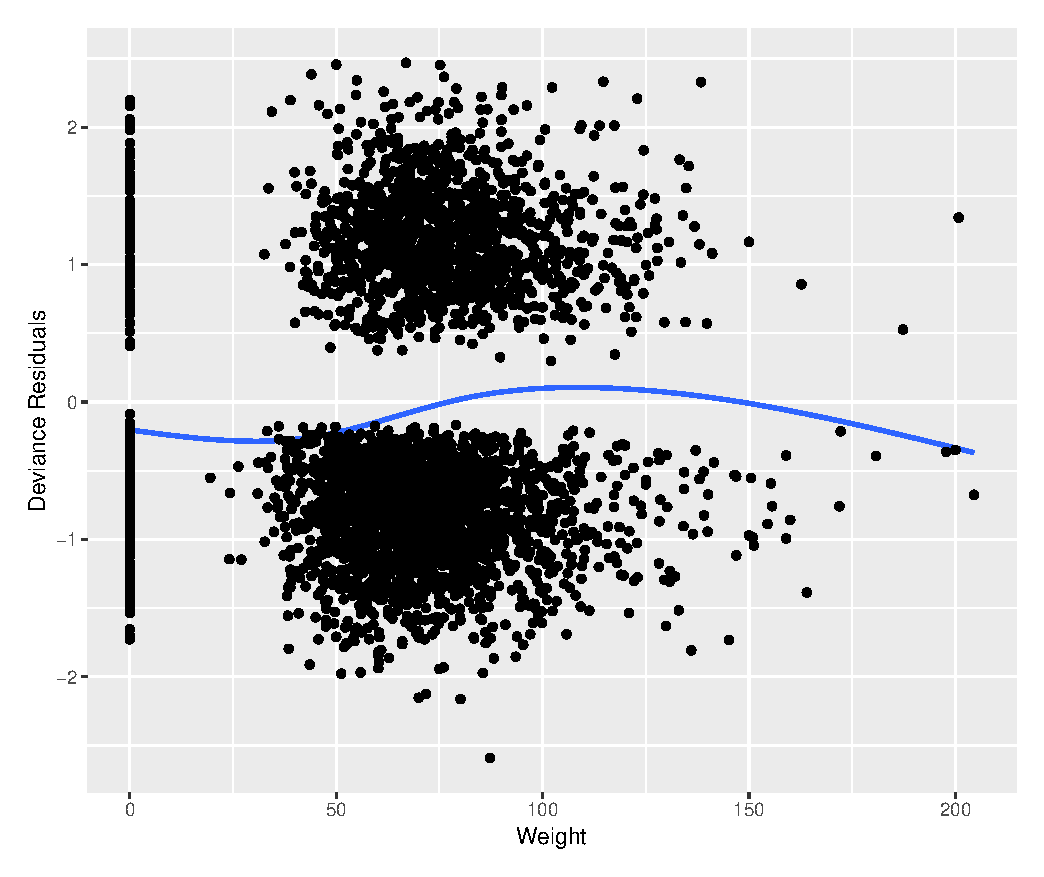
\includegraphics[width = \textwidth]{weight.eps}
	\caption{Deviance against weight}
	\end{subfigure}%
	\begin{subfigure}[b]{0.5\textwidth}
	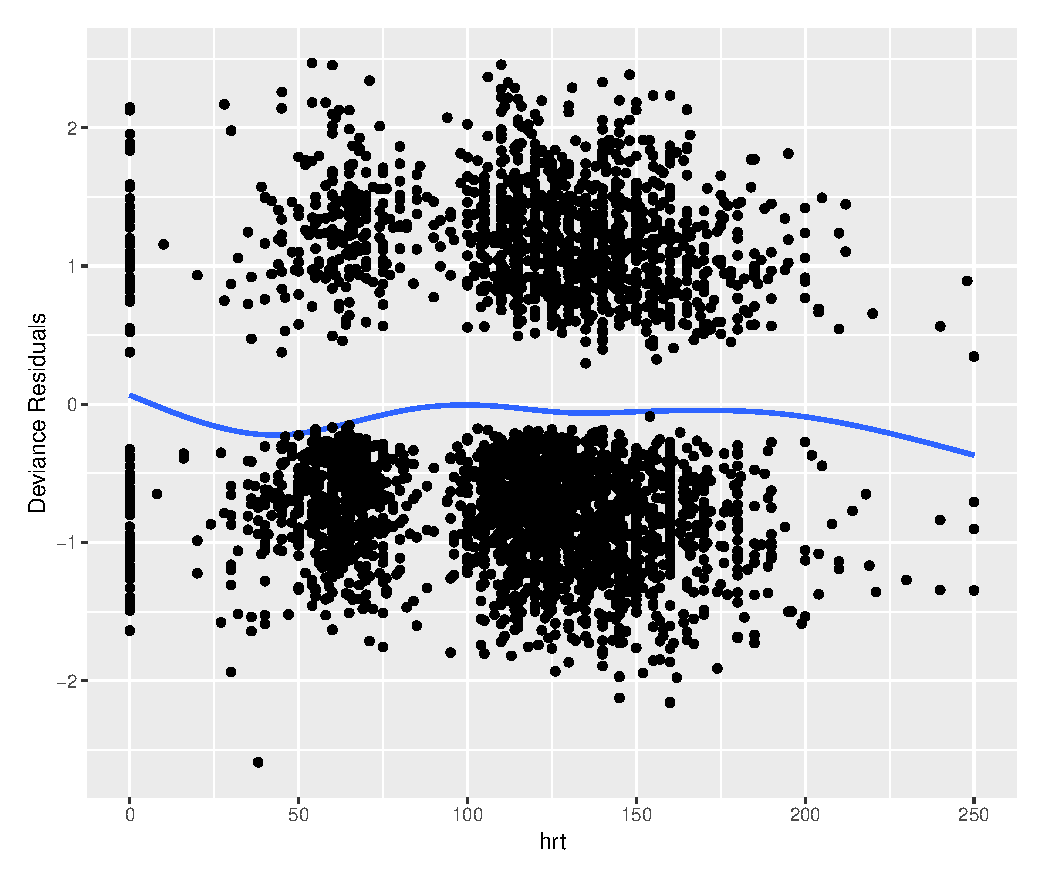
\includegraphics[width = \textwidth]{hrt.eps}
	\caption{Deviance against hrt}
	\end{subfigure}
	\caption{Deviance plot}
	\label{devp}
\end{figure}	


\newpage
ANOVA table for model3 is
\begin{verbatim}
             Df Deviance Resid. Df Resid. Dev  Pr(>Chi)    
     NULL                     3880     5129.5              
     edu      1   11.550      3879     5118.0 0.0006777 ***
     insur    5   26.417      3874     5091.6 7.405e-05 ***
     disease  3  218.443      3871     4873.1 < 2.2e-16 ***
     dnr      1   23.776      3870     4849.3 1.082e-06 ***
     cancer   2   29.802      3868     4819.5 3.377e-07 ***
     aps      1  178.015      3867     4641.5 < 2.2e-16 ***
     rrate    1  105.690      3866     4535.8 < 2.2e-16 ***
     pafi     1  157.533      3865     4378.3 < 2.2e-16 ***
     paco2    1   30.011      3864     4348.3 4.295e-08 ***
     pH       1    7.428      3863     4340.9 0.0064225 ** 
     hemat    1    7.658      3862     4333.2 0.0056512 ** 
     pot      1   17.475      3861     4315.7 2.910e-05 ***
     resp     1   32.645      3860     4283.1 1.107e-08 ***
     card     1   48.411      3859     4234.7 3.456e-12 ***
     neuro    1   41.525      3858     4193.2 1.164e-10 ***
     hema     1   10.319      3857     4182.8 0.0013167 ** 
     seps     1    8.980      3856     4173.9 0.0027290 ** 
     trauma   1    9.210      3855     4164.6 0.0024070 ** 
     ---
     Signif. codes:  0 ‘***’ 0.001 ‘**’ 0.01 ‘*’ 0.05 ‘.’ 0.1 ‘ ’ 1
\end{verbatim}

The summary of cross validated accuracies is
\begin{verbatim}
   Min. 1st Qu.  Median    Mean 3rd Qu.    Max. 
 0.6843  0.7055  0.7141  0.7144  0.7223  0.7564 
\end{verbatim}

So model3 still has pretty good classification ability. Thus we decide to use model3.

\subsection{Final model and conclusions}
The final model we chose is model3:
\begin{verbatim}
   y ~ edu + insur + disease + dnr + cancer + aps + rrate + pafi + 
       paco2 + pH + hemat + pot + resp + card + neuro + hema + seps + 
       trauma
\end{verbatim}

Parameter estimates and standard errors are
\begin{verbatim}
                   Estimate Std. Error z value Pr(>|z|)    
     (Intercept) 10.8753149  3.5097099   3.099  0.00194 ** 
     edu          0.0324512  0.0124989   2.596  0.00942 ** 
     insur2      -0.1987640  0.1763851  -1.127  0.25980    
     insur3      -0.1443279  0.1787596  -0.807  0.41944    
     insur4      -0.5121279  0.1983942  -2.581  0.00984 ** 
     insur5      -0.0548816  0.2215693  -0.248  0.80437    
     insur6       0.0872361  0.1718335   0.508  0.61168    
     disease2     0.4329258  0.1001886   4.321 1.55e-05 ***
     disease3     0.6830859  0.1598565   4.273 1.93e-05 ***
     disease4    -0.5615477  0.1224331  -4.587 4.51e-06 ***
     dnrYes      -0.6198725  0.1352844  -4.582 4.61e-06 ***
     cancer2      0.0077528  0.1774039   0.044  0.96514    
     cancer3      0.4328132  0.1099677   3.936 8.29e-05 ***
     aps          0.0214893  0.0025539   8.414  < 2e-16 ***
     rrate       -0.0269535  0.0029498  -9.137  < 2e-16 ***
     pafi        -0.0050261  0.0003956 -12.705  < 2e-16 ***
     paco2       -0.0201998  0.0041429  -4.876 1.08e-06 ***
     pH          -1.2765421  0.4517924  -2.826  0.00472 ** 
     hemat       -0.0146116  0.0052982  -2.758  0.00582 ** 
     pot         -0.1829244  0.0392112  -4.665 3.08e-06 ***
     resp1       -0.4150826  0.0912421  -4.549 5.38e-06 ***
     card1        0.5844181  0.0913362   6.399 1.57e-10 ***
     neuro1      -0.8373280  0.1470326  -5.695 1.23e-08 ***
     hema1       -0.5320483  0.1708819  -3.114  0.00185 ** 
     seps1        0.3304133  0.1053623   3.136  0.00171 ** 
     trauma1      1.1410598  0.3885272   2.937  0.00332 ** 
     ---
     Signif. codes:  0 ‘***’ 0.001 ‘**’ 0.01 ‘*’ 0.05 ‘.’ 0.1 ‘ ’ 1
\end{verbatim}

From the ANOVA table of model3, we find disease, aps, rrate and pafi are very important in this model. People with any one disease of ARF, MOSF or CHF has higher probability to receive RHC. And people with MOSF is more likely to receive RHC than people with ARF. People with CHF are more likely to receive RHC than people with MOSF. People with lower respiratory rate have higher probability to receive RHC. People with higher APACHE score have higher probability to receive RHC and people with lower $\mathrm{PaO}_2/\mathrm{FiO}_2$ ratio has higher probability to receive RHC.  We also find people with cancer have lower probability to receive RHC than people with no cancer. The years of education and insurance has a effect on the probability but not so much like other variables. Some of admission diagnosis can affect the probability: people with respiratory disease, Hematological disorder and neurological disease are less likely to receive RHC while people with cardiovascular disease, sepsis and trauma are more likely to receive RHC.

From the result of cross validation, we have about 70\% accuracy to classify patients with this model. The accuracy is not high, but I think that's the best we can do with this data set. And from the parameter estimates, I think the association between receiving RHC and variables in the model can make sense.


	
	\end{document}